
%% AHS_2017.tex
%% V1.4b
%% 2015/08/26
%% by Michael Shell
%% See:
%% http://www.michaelshell.org/
%% for current contact information.
%%
%% This is a skeleton file demonstrating the use of IEEEtran.cls
%% (requires IEEEtran.cls version 1.8b or later) with an IEEE
%% conference paper.
%%
%% Support sites:
%% http://www.michaelshell.org/tex/ieeetran/
%% http://www.ctan.org/pkg/ieeetran
%% and
%% http://www.ieee.org/

%%*************************************************************************
%% Legal Notice:
%% This code is offered as-is without any warranty either expressed or
%% implied; without even the implied warranty of MERCHANTABILITY or
%% FITNESS FOR A PARTICULAR PURPOSE! 
%% User assumes all risk.
%% In no event shall the IEEE or any contributor to this code be liable for
%% any damages or losses, including, but not limited to, incidental,
%% consequential, or any other damages, resulting from the use or misuse
%% of any information contained here.
%%
%% All comments are the opinions of their respective authors and are not
%% necessarily endorsed by the IEEE.
%%
%% This work is distributed under the LaTeX Project Public License (LPPL)
%% ( http://www.latex-project.org/ ) version 1.3, and 	may be freely used,
%% distributed and modified. A copy of the LPPL, version 1.3, is included
%% in the base LaTeX documentation of all distributions of LaTeX released
%% 2003/12/01 or later.
%% Retain all contribution notices and credits.
%% ** Modified files should be clearly indicated as such, including  **
%% ** renaming them and changing author support contact information. **
%%*************************************************************************


% *** Authors should verify (and, if needed, correct) their LaTeX system  ***
% *** with the testflow diagnostic prior to trusting their LaTeX platform ***
% *** with production work. The IEEE's font choices and paper sizes can   ***
% *** trigger bugs that do not appear when using other class files.       ***                          ***
% The testflow support page is at:
% http://www.michaelshell.org/tex/testflow/



\documentclass[conference]{IEEEtran}
% Some Computer Society conferences also require the compsoc mode option,
% but others use the standard conference format.
%
% If IEEEtran.cls has not been installed into the LaTeX system files,
% manually specify the path to it like:
% \documentclass[conference]{../sty/IEEEtran}





% Some very useful LaTeX packages include:
% (uncomment the ones you want to load)


% *** MISC UTILITY PACKAGES ***
%
%\usepackage{ifpdf}
% Heiko Oberdiek's ifpdf.sty is very useful if you need conditional
% compilation based on whether the output is pdf or dvi.
% usage:
% \ifpdf
%   % pdf code
% \else
%   % dvi code
% \fi
% The latest version of ifpdf.sty can be obtained from:
% http://www.ctan.org/pkg/ifpdf
% Also, note that IEEEtran.cls V1.7 and later provides a builtin
% \ifCLASSINFOpdf conditional that works the same way.
% When switching from latex to pdflatex and vice-versa, the compiler may
% have to be run twice to clear warning/error messages.






% *** CITATION PACKAGES ***
%
%\usepackage{cite}
% cite.sty was written by Donald Arseneau
% V1.6 and later of IEEEtran pre-defines the format of the cite.sty package
% \cite{} output to follow that of the IEEE. Loading the cite package will
% result in citation numbers being automatically sorted and properly
% "compressed/ranged". e.g., [1], [9], [2], [7], [5], [6] without using
% cite.sty will become [1], [2], [5]--[7], [9] using cite.sty. cite.sty's
% \cite will automatically add leading space, if needed. Use cite.sty's
% noadjust option (cite.sty V3.8 and later) if you want to turn this off
% such as if a citation ever needs to be enclosed in parenthesis.
% cite.sty is already installed on most LaTeX systems. Be sure and use
% version 5.0 (2009-03-20) and later if using hyperref.sty.
% The latest version can be obtained at:
% http://www.ctan.org/pkg/cite
% The documentation is contained in the cite.sty file itself.






% *** GRAPHICS RELATED PACKAGES ***
%
\ifCLASSINFOpdf
\usepackage[pdftex]{graphicx}
  % declare the path(s) where your graphic files are
  % \graphicspath{{../pdf/}{../jpeg/}}
  % and their extensions so you won't have to specify these with
  % every instance of \includegraphics
  % \DeclareGraphicsExtensions{.pdf,.jpeg,.png}
\else
  % or other class option (dvipsone, dvipdf, if not using dvips). graphicx
  % will default to the driver specified in the system graphics.cfg if no
  % driver is specified.
  % \usepackage[dvips]{graphicx}
  % declare the path(s) where your graphic files are
  % \graphicspath{{../eps/}}
  % and their extensions so you won't have to specify these with
  % every instance of \includegraphics
  % \DeclareGraphicsExtensions{.eps}
\fi
% graphicx was written by David Carlisle and Sebastian Rahtz. It is
% required if you want graphics, photos, etc. graphicx.sty is already
% installed on most LaTeX systems. The latest version and documentation
% can be obtained at: 
% http://www.ctan.org/pkg/graphicx
% Another good source of documentation is "Using Imported Graphics in
% LaTeX2e" by Keith Reckdahl which can be found at:
% http://www.ctan.org/pkg/epslatex
%
% latex, and pdflatex in dvi mode, support graphics in encapsulated
% postscript (.eps) format. pdflatex in pdf mode supports graphics
% in .pdf, .jpeg, .png and .mps (metapost) formats. Users should ensure
% that all non-photo figures use a vector format (.eps, .pdf, .mps) and
% not a bitmapped formats (.jpeg, .png). The IEEE frowns on bitmapped formats
% which can result in "jaggedy"/blurry rendering of lines and letters as
% well as large increases in file sizes.
%
% You can find documentation about the pdfTeX application at:
% http://www.tug.org/applications/pdftex
\usepackage{amsmath} % assumes amsmath package installed
\usepackage{amssymb}  % assumes amsmath package installed
\usepackage{balance}
%\usepackage{amsxtra}
%\usepackage{amsfonts}
\usepackage{graphics} % for pdf, bitmapped graphics files
%\usepackage{epsfig} % for postscript graphics files
%\usepackage{float}
\usepackage{graphicx}
%\usepackage{caption}
%\usepackage{setspace}
\usepackage{color}
\usepackage{subfigure}
%\usepackage{subfig}
%\usepackage{psfrag}
%\usepackage{dsfont}
\usepackage{multirow}
%\usepackage{algorithm}
%\usepackage{algorithmic}
\usepackage{todonotes}
\usepackage{url}
\usepackage{hyperref}
\usepackage{bm}


\newcommand{\Ne}{\mathbb {N}}




\usepackage{hyperref}



% *** MATH PACKAGES ***
%
\usepackage{amsmath}
% A popular package from the American Mathematical Society that provides
% many useful and powerful commands for dealing with mathematics.
%
% Note that the amsmath package sets \interdisplaylinepenalty to 10000
% thus preventing page breaks from occurring within multiline equations. Use:
%\interdisplaylinepenalty=2500
% after loading amsmath to restore such page breaks as IEEEtran.cls normally
% does. amsmath.sty is already installed on most LaTeX systems. The latest
% version and documentation can be obtained at:
% http://www.ctan.org/pkg/amsmath
\usepackage{amsthm}

%\usepackage{subcaption}
\usepackage{graphicx}
\graphicspath{ {fig/} }
%\usepackage{subfigure}
% *** SPECIALIZED LIST PACKAGES ***
%
%\usepackage{algorithm}
%\usepackage{algorithmic}
\usepackage[linesnumbered,ruled]{algorithm2e}
% algorithmic.sty was written by Peter Williams and Rogerio Brito.
% This package provides an algorithmic environment fo describing algorithms.
% You can use the algorithmic environment in-text or within a figure
% environment to provide for a floating algorithm. Do NOT use the algorithm
% floating environment provided by algorithm.sty (by the same authors) or
% algorithm2e.sty (by Christophe Fiorio) as the IEEE does not use dedicated
% algorithm float types and packages that provide these will not provide
% correct IEEE style captions. The latest version and documentation of
% algorithmic.sty can be obtained at:
% http://www.ctan.org/pkg/algorithms
% Also of interest may be the (relatively newer and more customizable)
% algorithmicx.sty package by Szasz Janos:
% http://www.ctan.org/pkg/algorithmicx




% *** ALIGNMENT PACKAGES ***
%
%\usepackage{array}
% Frank Mittelbach's and David Carlisle's array.sty patches and improves
% the standard LaTeX2e array and tabular environments to provide better
% appearance and additional user controls. As the default LaTeX2e table
% generation code is lacking to the point of almost being broken with
% respect to the quality of the end results, all users are strongly
% advised to use an enhanced (at the very least that provided by array.sty)
% set of table tools. array.sty is already installed on most systems. The
% latest version and documentation can be obtained at:
% http://www.ctan.org/pkg/array


% IEEEtran contains the IEEEeqnarray family of commands that can be used to
% generate multiline equations as well as matrices, tables, etc., of high
% quality.




% *** SUBFIGURE PACKAGES ***
%\ifCLASSOPTIONcompsoc
%  \usepackage[caption=false,font=normalsize,labelfont=sf,textfont=sf]{subfig}
%\else
%  \usepackage[caption=false,font=footnotesize]{subfig}
%\fi
% subfig.sty, written by Steven Douglas Cochran, is the modern replacement
% for subfigure.sty, the latter of which is no longer maintained and is
% incompatible with some LaTeX packages including fixltx2e. However,
% subfig.sty requires and automatically loads Axel Sommerfeldt's caption.sty
% which will override IEEEtran.cls' handling of captions and this will result
% in non-IEEE style figure/table captions. To prevent this problem, be sure
% and invoke subfig.sty's "caption=false" package option (available since
% subfig.sty version 1.3, 2005/06/28) as this is will preserve IEEEtran.cls
% handling of captions.
% Note that the Computer Society format requires a larger sans serif font
% than the serif footnote size font used in traditional IEEE formatting
% and thus the need to invoke different subfig.sty package options depending
% on whether compsoc mode has been enabled.
%
% The latest version and documentation of subfig.sty can be obtained at:
% http://www.ctan.org/pkg/subfig




% *** FLOAT PACKAGES ***
%
%\usepackage{fixltx2e}
% fixltx2e, the successor to the earlier fix2col.sty, was written by
% Frank Mittelbach and David Carlisle. This package corrects a few problems
% in the LaTeX2e kernel, the most notable of which is that in current
% LaTeX2e releases, the ordering of single and double column floats is not
% guaranteed to be preserved. Thus, an unpatched LaTeX2e can allow a
% single column figure to be placed prior to an earlier double column
% figure.
% Be aware that LaTeX2e kernels dated 2015 and later have fixltx2e.sty's
% corrections already built into the system in which case a warning will
% be issued if an attempt is made to load fixltx2e.sty as it is no longer
% needed.
% The latest version and documentation can be found at:
% http://www.ctan.org/pkg/fixltx2e


%\usepackage{stfloats}
% stfloats.sty was written by Sigitas Tolusis. This package gives LaTeX2e
% the ability to do double column floats at the bottom of the page as well
% as the top. (e.g., "\begin{figure*}[!b]" is not normally possible in
% LaTeX2e). It also provides a command:
%\fnbelowfloat
% to enable the placement of footnotes below bottom floats (the standard
% LaTeX2e kernel puts them above bottom floats). This is an invasive package
% which rewrites many portions of the LaTeX2e float routines. It may not work
% with other packages that modify the LaTeX2e float routines. The latest
% version and documentation can be obtained at:
% http://www.ctan.org/pkg/stfloats
% Do not use the stfloats baselinefloat ability as the IEEE does not allow
% \baselineskip to stretch. Authors submitting work to the IEEE should note
% that the IEEE rarely uses double column equations and that authors should try
% to avoid such use. Do not be tempted to use the cuted.sty or midfloat.sty
% packages (also by Sigitas Tolusis) as the IEEE does not format its papers in
% such ways.
% Do not attempt to use stfloats with fixltx2e as they are incompatible.
% Instead, use Morten Hogholm'a dblfloatfix which combines the features
% of both fixltx2e and stfloats:
%
% \usepackage{dblfloatfix}
% The latest version can be found at:
% http://www.ctan.org/pkg/dblfloatfix




% *** PDF, URL AND HYPERLINK PACKAGES ***
%
%\usepackage{url}
% url.sty was written by Donald Arseneau. It provides better support for
% handling and breaking URLs. url.sty is already installed on most LaTeX
% systems. The latest version and documentation can be obtained at:
% http://www.ctan.org/pkg/url
% Basically, \url{my_url_here}.

% *** Do not adjust lengths that control margins, column widths, etc. ***
% *** Do not use packages that alter fonts (such as pslatex).         ***
% There should be no need to do such things with IEEEtran.cls V1.6 and later.
% (Unless specifically asked to do so by the journal or conference you plan
% to submit to, of course. )


% correct bad hyphenation here
\hyphenation{op-tical net-works semi-conduc-tor}

\newtheorem{problem}{Problem}
\newtheorem{theorem}{Theorem}[section]
\newtheorem{corollary}{Corollary}[theorem]
\newtheorem{lemma}[theorem]{Lemma}
\newcommand*{\affaddr}[1]{#1} % No op here. Customize it for different styles.
\newcommand*{\affmark}[1][*]{\textsuperscript{#1}}
\newcommand*{\email}[1]{\texttt{#1}}

\newcommand\NB[1]{$\spadesuit$\footnote{NB: #1}}
\newcommand\JL[1]{$\diamondsuit$\footnote{MH: #1}}
\newcommand\ME[1]{$\spadesuit$\footnote{ME: #1}}

%\renewcommand{\algorithmicrequire}{\textbf{Input:}}
%\renewcommand{\algorithmicensure}{\textbf{Output:}}
%\newcommand{\algorithmicbreak}{\textbf{break}}
%\newcommand{\BREAK}{\STATE \algorithmicbreak}

%\renewcommand{\baselinestretch}{0.95}

\begin{document}

\title{Cyber-Physical Attack Intention Prediction and Recovery} 
% affiliations

\author{\IEEEauthorblockN{Mahmoud Elnaggar\affmark[1],
 and Nicola Bezzo\affmark[1,2]}
\IEEEauthorblockA{\affmark[1]Department of Systems and Information Engineering\\
\affmark[2]Department of Electrical and Computer Engineering\\
University of Virginia\\
Email: \{mae3tb,nbezzo\}@virginia.edu}}


% make the title area
\maketitle

% in the abstract
\begin{abstract}
\end{abstract}

% For peer review papers, you can put extra information on the cover
% page as needed:
% \ifCLASSOPTIONpeerreview
% \begin{center} \bfseries EDICS Category: 3-BBND \end{center}
% \fi
%
% For peerreview papers, this IEEEtran command inserts a page break and
% creates the second title. It will be ignored for other modes.
\IEEEpeerreviewmaketitle



\section{Introduction}
\NB{iPlease use the correct ACC template}
\NB{I rewrote the intro. It was very confusing and it looks more a news report}
The majority of modern cyber-physical systems (CPSs) are not built with cybersecurity in mind. The tight coupling between information technology and the physical world have introduced security vulnerabilities in the form of physical and cyber attacks (e.g., sensor, actuator, controller, communication and environment attacks).
%Cyber-Physical security has grasped a lot of attention in the research community specially during the last decade. 
Multiple incidents that have occurred recently indicate the ability of a malicious attacker to compromise modern cyber-physical systems using different techniques. For example, the well known StuxNet cyber attack on an Iranian nuclear reactors in 2011 was performed by exploiting five zero-day vulnerabilities in the Operating Systems installed on the computers that operate the SCADA system to control the nuclear centrifuges \cite{langner_2013}. This type of attack operated at a cyber level targeting the physical plant by leveraging the knowledge on how the system was being operated and controlled. Cyber-attacks on modern automobiles have also been widely explored like in \cite{} in which the hackers were able to take over different  system components and hijack the vehicle by tempering with its infotainment system.
%Another type of attacks on a cyber-physical system is the one that operates on the system control level, with the aim to exploit vulnerabilities in the system by compromising different components of the control system.

A typical CPS contains multiple buses/networks that connect sensors and actuators with controllers, data storage and processing units, and human machine interfaces. More precisely it consists of: a) controllers, b) networking devices and buses, c) sensors, s) actuators, and d) the physical plant. An attacker can compromise the operation of a CPS by attacking any of these components. 

In this paper we focus on sensor attacks, specifically sensor spoofing in which a malicious program masquerades as another sensor by falsifying data while staying stealthy within the error noise of the sensor measurement. GPS spoofing in particular has been demonstrated in several works \cite{humphreys2008assessing, protecting_gps_2016, peterson_faramarzi_2011}. A malicious attacker can use a hand-held device to deceive a GPS receiver by broadcasting signals synchronized with the genuine signals observed by the target receiver. The power of the counterfeit signals is then gradually increased and drawn away from the genuine signals \cite{humphreys2008assessing}. Such attack has been demonstrated on different vehicles compromising their safety and/or hijacking them to undesired states.
%
%If this type of attack is exploited on a dynamic CPS like an unmanned ground vehicle (UGV) or an unmanned aerial vehicle (UAV) that is navigating to a desired destination, it can make the autonomous vehicle crash or get hijacked and sent to an undesired location.
%
%One of the most widely used sensors for localization is the GPS. It has been shown in \cite{humphreys2008assessing} that a typical GPS is vulnerable to sensor spoofing attacks. A malicious attacker can use a hand-held device to deceive the GPS receiver in a system by broadcasting incorrect GPS signals. 
%If this type of attacks is performed on a dynamic cyber-physical system i.e. a UGV (Unmanned Ground Vehicle) or a UAV (Unmanned Aerial Vehicle) that is navigating to a desired destination, it can make the autonomous vehicle crash or get hijacked and sent to an undesired location
For example, it is believed that GPS spoofing leaded to the capturing of a Sentinel drone in Iran in 2011 \cite{peterson_faramarzi_2011}. More recently, researchers in \cite{protecting_gps_2016} have also demonstrated a GPS spoofing attack on a vessel, making it deviate from its desired course.
 
%An example that shows how the impact of GPS spoofing can be drastic is the American UAV hijacking incident in 2011. According to \cite{peterson_faramarzi_2011} the autonomous drone was supposed to land in Afghanistan and the attacker sent false positions to the drone via GPS spoofing to deceive the autonomous controller and make it land in Iran instead of Afghanistan. The US government acknowledged losing the control of the drone but it didn't confirm whether it happened due to a GPS spoofing attack or not. Another example of GPS spoofing attacks was demonstrated by researchers from University of Texas and Cornell University, when they conducted an attack by spoofing the GPS receiver on a \$80 million vessel cruising in the Mediterranean sea. The attack made the vessel go off the desired course while thinking it is still following the correct coarse \cite{protecting_gps_2016}.

\begin{figure}[h]
\centering
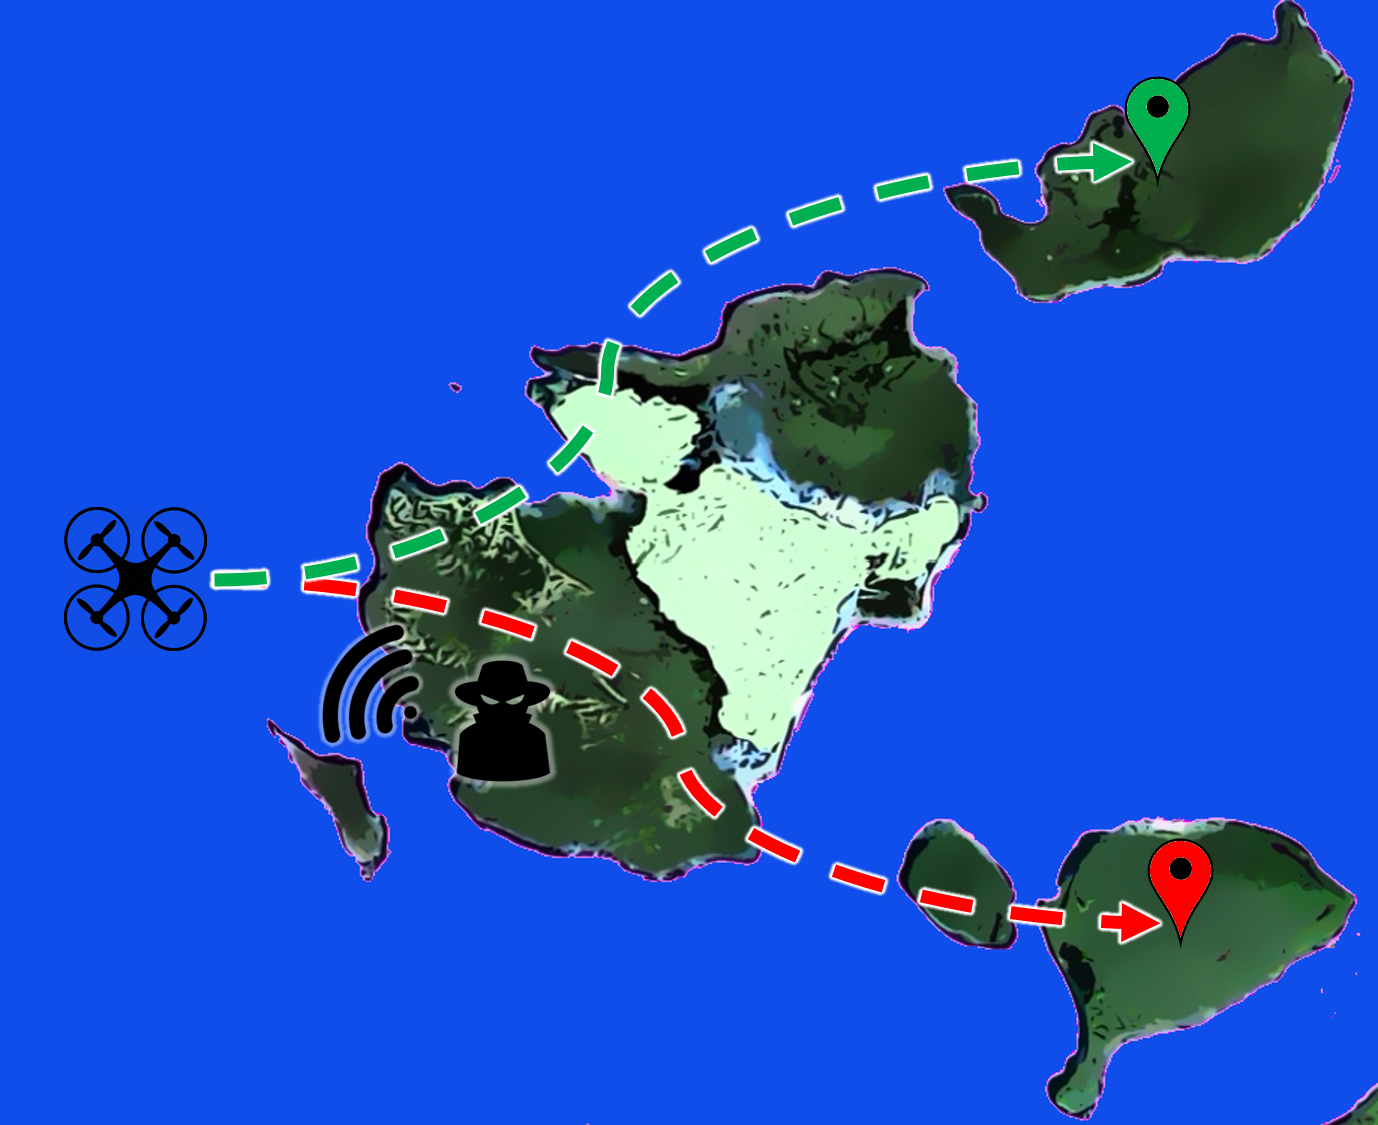
\includegraphics[width=0.5\textwidth]{problem}
\caption{A malicious attacker spoofs UAV's  GPS receiver to drive it to an undesired destination instead of its original one}
 \label{fig:problem}
\end{figure}

In this paper, we are interested in addressing similar problems as the one illustrated in Fig.\ref{fig:problem}. We consider the case where an autonomous vehicle, equipped with multiple sensors, is tasked to perform a go-to-goal navigation. 
%The state estimator of the autonomous vehicle uses a number of sensors to estimate its position. 
%We assume that the vehicle has at least one sensor that is not vulnerable to spoofing attacks or in other words, the attacker is not able to spoof at least one sensor. 
A malicious attacker performs a coordinated attack by spoofing one or more of sensors on the vehicle. The goal of the attacker is to drive the vehicle to a different destination than its original destination while hiding within the sensor and actuator noise profile and disturbance model of the system. 
%The attacker's desired destination can be a hostile territory to the vehicle, or an obstacle that will make the vehicle crash if it hits it. 
%We consider a smart attacker who hides his sensor attack vectors within the noise profiles of the attacked sensors or within the environment disturbance model.

Our goal is to develop a technique to infer the intention of the attacker and recover the system before reaching the undesired state. 
The intuition is that if we are able to determine which set of sensors are under attack before the vehicle arrives to the undesired destination, we can correctly reconstruct the state of the vehicle using the remaining uncompromised set of sensors. 

\NB{you need to add the approach that we are using and contribution here}
%Once the vehicle state is estimated correctly, the controller can drive the vehicle back on its coarse navigating towards the desired destination.

\subsection{Related Work}\label{subsec:related}
\NB{related work needs to be rewritten in a different way without subsections. You need to introduce our proposed work before talking about related work in IRL. The first part of the related work needs to be expanded. Do not condensate multiple papers together. Expand each paper description. After that introduce that in this work we will use machine learning techniques and that they have not been explored too much in the literature on CPS cyber-security. Refer to my ACC paper on ROMPD and then describe related work on RL and IRL.}

\subsubsection{Resilient State Estimators}

Various efforts have been done by members of the research community to guarantee the safety of cyber-physical system under sensor attacks. A major contribution was done by developing secure and resilient state estimators of cyber-physical systems. The results presented in \cite{Fawzi2014,Ivanov2014,Pajic2014,Pajic2017} show that by using redundant sensors in a system, and leveraging the knowledge of the system model, the secure state estimators are able to correctly estimate the state of the system if the number of attacked sensors is less than half of the number of the sensors. An important assumption that these works considered is that the sensor attack vectors don't hide within the noise profiles of the sensors nor the environment disturbance model. Given this assumption, the resilient state estimator can not only correctly estimate the state of a compromised system, but also it can tell which sensors are under attack and which are not by comparing sensor readings with system model.

In our case, we assume that the attacker hides his attack vectors within the noise profiles of the system sensors, which means we need to develop a new technique to detect which set of sensors are under attack after we detect that an attack is happening. We leverage state-of-the-art Inverse Reinforcement Learning (IRL) techniques to infer the desired destination of the attacker and at the same time detect which sensors are compromised.

\subsubsection{Inverse Reinforcement Learning}
The problem of Inverse Reinforcement Learning has been addressed in multiple domains. It was first introduced in \cite{Ng2000}. An algorithm for apprenticeship learning via IRL was introduced in \cite{Abbeel2004a} where the authors considered the case where the reward function is expressible as a linear combination of known features. IRL problem was first cast as a Bayesian inference problem in  \cite{Ramachandran2007}. It was shown that there Bayesian Inverse Reinforcement Learning (BIRL) algorithm can be used for reward learning and also policy learning. Policy walk algorithm was also introduced which is based on Monte Carlo Marcov Chain (MCMC) algorithm. Michini et al. \cite{Michini2015,Michini2013,Michini2012} extended BIRL algorithm to deal with continuous state and action spaces and introduced the Non-Parametric Bayesian Inverse Reinforcement Learning (BNIRL) algorithm. They  showed that by observing a UAV performing different maneuvers in a continuous 3D space. The BNIRL algorithm was able to infer what are the intermediate goals and the final goal that the observed UAV was trying to reach. They used this predicted information to make another UAV perform the same observed maneuvers.

The previous works considered the case where we can observe a moving agent completing its desired trajectory from source to destination. In other applications, we may want to observe the agent navigating in the environment and try to predict its future trajectory and its desired destination. In this case, we have partial set of observation. This problem was studied in \cite{Best2015} where they used Bayesian Inference to predict the intention of an agent navigating in a partially occluded environment. The intention of the agent was represented by the goal the agent is trying to reach based on the assumption that the agent will most likely take the shortest path to the goal position, with some uncertainty in its transition model.

In the cyber-physical literature, to our knowledge, no research has been done so far that uses IRL to predict the intention of an attacker.

\NB{Conclude related work with a summary about the organization of the paper: i.e., in Section III, we present ..., in section .... etc }.
%The idea of check-pointing and recovery has been applied to many computing systems \cite{Zhang2003,Processors2017,Koo1987, Prakash1996}. By taking snapshots of the state of a system in a cyclic fashion or after the occurrence of specific events, we can roll-back to the last saved checkpoint if a fault occurs to recover the system from that fault. This technique cannot be directly applied to a dynamical system without modifying the definitions of a checkpoint and a roll-back for two reasons. 
%\begin{enumerate}
    %\item This technique assumes that every checkpoint we take represents a correct state of the system. For a dynamical system under sensor attack, detection of an attack doesn't occur immediately after an attack starts. Which means that the saved checkpoints between the time the attack started and the time it is detected are considered incorrect states. For that matter, we need to consider the fact that we can have correct and incorrect checkpoints in the system and the the recovery mechanism shall find the last correct checkpoint in the system.
    %\item Roll-back is considered successful when the last checkpoint is recovered. For a dynamical system which moves in the physical space. To tolerate a fault or mitigate an attack, the recovery process is considered success-full when the correctly estimate the state of the system, not necessarily by returning back to the last saved correct check-point. Thus, the role of the recovery mechanism in our case is to find what is the last correct checkpoint, and use this information to determine the current state of the system correctly.
%\end{enumerate}

\section{Preliminaries}\label{sec:Preliminaries}
In this paper, we provide a solution that uses Bayesian Inverse Reinforcement Learning techniques inside a Markov Decision Process (MDP) environment.\NB{What? You are providing preliminaries that will be used in the next sections, not a solution} This section provides the foundations from MDP and IRL that our approach relies on\NB{rewrite, incorrect and contorted english}.
\subsection{Markov Decision Process}
A finite state Markov Decision Process (MDP) \cite{puterman2014markov} consists of a tuple $(S,A,T,R,\gamma)$ where:
\begin{itemize}
    \item The set $S$ is the set of all the states \NB{why are you repeating set twice...go directly to the point. S is the set of all...}.
    \item The set $A$ is the set of all possible actions.
    \item The function $T : S\times A\times S \mapsto [0,1]$ is the transition probabilities function. $T(s,a,s')$ is the probability that moving to state $s'$ from state $s$ after action $a$ is taken.
    \item The reward function $R$ can be a function of the state only $R(s)$, a function of states and actions $R(s,a)$, or a function of the states, actions, and the next states $R(s,a,s')$.
    \item The discount factor $\gamma$ is the factor that the reward function gets discounted with over time.
\end{itemize}
To solve and MDP problem, we are interested in finding an optimal stationary policy $\pi^*: S \mapsto A$ that maximizes the expected value of the discounted future rewards.
In order to find $\pi^*$, we need to define a value function for all state $s \in S$ given a reward function $R(s)$ and a policy $\pi$ as follows:
\[ V^\pi(s,R) = R(s) + \sum_{s'}^{}\gamma\,T(s,\pi(s),s')\,V^\pi(s') \]
The value function of state $s$ is equal to the reward received in state $s$ plus the sum of the discounted expected value function for each neighbor state $s'$ when actions are taken according to the policy $\pi$.
We need also to define \NB{why we need this?} a function that evaluates the value of taking action $a$ for each state $s$ which is called the Q-function.
\[Q^\pi(s,a,R) = R(s) + \sum_{s'}{} \gamma\,T(s,a,s')\,V^\pi(s') \]
Then, a policy $\pi$ is optimal iff, for each state $s \in S$:
\[ \pi(s) = \arg\!\max_{a\in A} Q^\pi(s,a,R)\]
The optimal policy $\pi^*$ corresponds to a state value function $V^*$ and a state-action value function $Q^*$.

\subsection{Reinforcement Learning}
\NB{why are you introducing RL? A reader here will be very confused if you don't connect this with the rest of the paper} Reinforcement Learning provides the notion of an agent that navigates the states of MDP environment by taking and an action $a \in A$. \NB{What??? RL provides the notion? What does it mean?} The agent receives a reward $r$ when it transitions from a state $s$ to state $s'$ by taking action $a$. The reward $r$ can take any of the three forms described earlier\NB{rewrite, very confusing.} . The task of Reinforcement Learning algorithms is to learn the optimal policy $\pi^*$ that maximizes the future expected rewards for the agent from its history of interaction with the environment. The history of the interactions can be formulated as a set of the tuple $\big \langle s,a,r,s' \big \rangle$
\subsection{Inverse Reinforcement Learning}
\NB{why are you introducing IRL? A reader here will be very confused if you don't connect this with the rest of the paper} In Inverse Reinforcement Learning (IRL), we consider an agent acting optimally or sub-optimally in an MDP environment. The agent is following an optimal or sub-optimal policy $\pi^a(s)$. The policy of the agent $\pi^a(s)$ can be observed as a set of state-action pairs $\{(s_1,a1),(s_2,a_2), ...,(s_N,a_N)\}$, where $N$ is the number of observations. The goal of IRL is to infer the reward function $R$ that is responsible for generating these observations. As mentioned before, $R$ can take on the three forms we described before\NB{confusing. What 3 forms?}.\NB{both this and the previous sections are too brief. Either we add some mathematical formulation that will be used next or we may have to remove or combine with another section}

\section{Problem Statement}\label{sec:problem}
We consider an autonomous vehicle that performs a navigation task to a desired destination in a stochastic environment. The vehicle has a set of sensors $\mathcal{S}$ where $|\mathcal{S}|=N$ \NB{Why this notation? just write: The vehicle is equipped with N sensors $s \in S$}. The readings from the $N$ sensors are fused together to estimate the state of the vehicle. We also consider a malicious attacker that can spoof a subset of sensors $\mathcal{S'}$ where $\mathcal{S'} \subset \mathcal{S}$, $|\mathcal{S'}| < N$. The goal of the attacker is to drive the vehicle towards an undesired destination while hiding its attack vectors within the noise profiles of the spoofed vehicle sensors or hiding it within the disturbance model of the stochastic environment. \NB{rewrite next section: Fig. \ref{fig:sensor_spoofing} summarizes the situation in which an attack is stealthily beginning at $t_1$...}
The attack begins at time $t_1$. The attack can stay stealthy to the system until the noise margins of the spoofed sensors don't overlap anymore with the noise margins of the uncompromised ones at $t_2$ as shown in Fig. \ref{fig:sensor_spoofing}. From $t_2$, an attack or fault can be detected due to the divergence in sensor readings. At this point, it is hard to distinguish between the compromised and uncompromoised sensors, as all sensor readings comply with the uncertainty model of the vehicle dynamics and the environment. .
\begin{figure}[h]
\centering
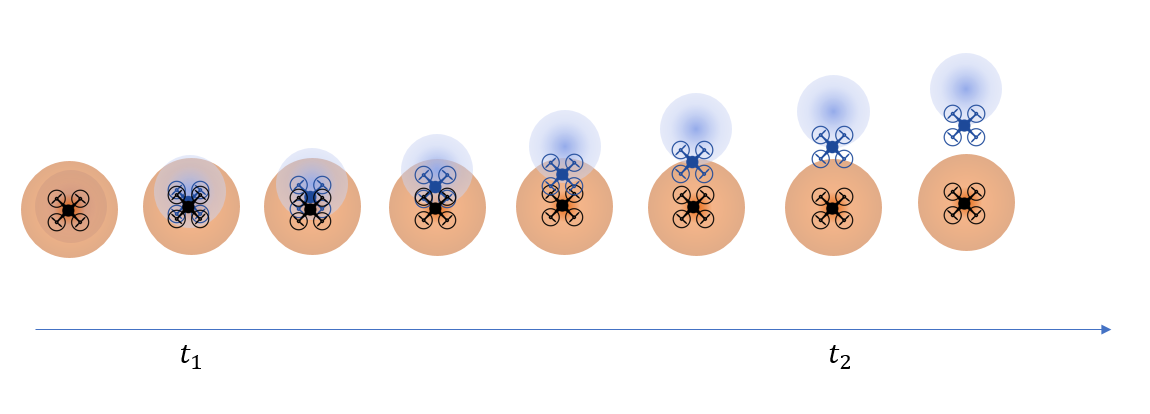
\includegraphics[width=0.5\textwidth]{sensor_spoofing}
\caption{An attack on the blue sensor starts at $t_1$. The attack can be detected at $t_2$ when the sensors error margins don't overlap anymore.}
 \label{fig:sensor_spoofing}
\end{figure}

Formally, We are interested in solving the following problem:

Problem 1 \NB{use latex environment to write problems} Attacker Intention Inference and Recovery: Consider the set $\mathcal{G}$ is the set of states that are considered undesired. Consider a super-set of observations $\mathcal{O}_{t_2:t} = \{\mathcal{O}_1, \mathcal{O}_2, ..., \mathcal{O}_N\}$, where $\mathcal{O}_{i,t_2:t} = \{(s_{i,t_2}, a_{t_2}), (s_{i,t_2+1}, a_{t_2+1}), ..., (s_{i,t_2+t}, a_{t_2+t})\}$ is the finite set of measurement-action pairs for each sensor $i$ which includes the history of sensor data recorded starting from the beginning of the attack detection time  $t = t_2$ until the current time $t$. We assume the attacker's goal is to drive the vehicle towards a target goal $g^a \in \mathcal{G}$. Where, $\mathcal{G}$ is the set of all possible undesired goals known a priori. Our goal is to recover from this attack. In order to do so, we need to infer the intention of the attacker by estimating their desired goal $g^a$ and determine the subset of compromised sensors $\mathcal{S'}$. \NB{Problem needs to be rewritten more formally. Given a set of undesired goals...a set of observations/actions ... and assume that a subset of observations...is compromised at a certain time t, find a policy to predict the intended goal of the attack and recover the system}

\section{Attacker Intention Inference}\label{sec:intpredic}
We propose to cast Problem 1 as Inverse Reinforcement Learning problem. In this problem, we consider the compromised autonomous vehicle under attack acts as an agent that navigates in the environment according to a policy $\pi^a$ \NB{is $\pi_a$ the policy of the attacker?}. The policy $\pi^a$ drives the agent towards the target destination $g^a$ as fast as possible while hiding the attack within the sensors noise profiles or the environment disturbance model. At each state $s$, the policy $\pi^a$ is calculated according to \NB{rewrite as follows: first introduce the optimal policy of the vehicle without attack. Then describe the optimal policy of the attacker.}:
\[ \pi^a(s) = \arg\!\max_{a\in A} Q^{\pi^a}(s,a,R^a)\]

The reward function $R^a$ can take many forms. For the sake of simplicity we assume the reward function $R^a$ that makes the agent moves towards the target goal $g$ can be modelled as follows \NB{confusing and unecessary. rewrite as follows: where $R^a$ is:}. 
  \begin{equation}
    R^a(s)=\left\{
                \begin{array}{ll}
                  c\hspace{2em} s = g\\
                  0\hspace{2em} s \ne g
                \end{array}
              \right.
  \end{equation}
Where $c$ is a positive constant.
\subsection{Bayesian Inference Reinforcement Learning}
Given the set of observations $\mathcal{O}_{t_2:t}$, the goal is to infer the intention of the attacker by inferring the reward function $R(s)$ the vehicle is trying to maximize. As attacker can compromise only a subset of sensors $\mathcal{S}'$, we use rely on this assumption to perform attacker's intention inference \NB{read and correct grammar}. Our intuition is that we can use the sensor readings of the compromised set of sensors and the actions taken by the vehicle to infer that they match the actions of the attacker's policy $\pi_a$ \NB{rewrite. This is very important. We are leveraging the history of past actions/sensor measurements and comparing with multiple optimal policies for each goals to infer the intention}. We propose a method that examines all the sensor readings and vehicle actions at the time the attack is detected $t_2$ \NB{instread of $t_2$ use a more formal notation like $t_d$. The same for $t_1$}. The goal is to search for the subset of the compromised sensors $\mathcal{S}'$  that cause the vehicle to drift towards the bad goal. The algorithm we propose leverages Bayesian Inverse Reinforcement Learning techniques (BIRL)\cite{Ramachandran2007} in order to do the inference. In BIRL, the inference of the reward function posterior $Pr(R|O)$ is a function of the reward function prior $Pr(R)$ and the likelihood of the observations $Pr(O|R)$ as follows:
\begin{equation} 
    Pr(R|O) = \frac{Pr(O|R)Pr(R)}{Pr(O)}
\end{equation}
Where, $Pr(O)$ is the probability distribution of $O$\NB{what is O? Write the formula above directly with our notation} over the entire space of reward function $R$. The normalization constant $Pr(O)$ is usually hard to compute as it requires performing multiple integral calculations which is usually not feasible to compute analytically. 

\NB{I changed a few things in what follows to make it flow a little bit betetr}To estimate the posterior distribution while avoiding calculating $Pr(O)$, we leverage the MCMC sampling algorithm presented in \cite{andrieu2003introduction} that allows to estimate of the distribution of the posterior $Pr(\tilde{R}|O)$. Since this is an estimation problem, we are interested in finding the value of $R$ that minimizes the expected Least Square Error (LSE) of the estimate $E[(R-\tilde{R})^2]$. It was proven in \cite{Ramachandran2007} that the mean of the estimated posterior distribution is the optimal estimator in that case. \NB{not clear this sentence. I didn't change it but I'm not able to understand if what comes next is an approach to find the mean?? }

In order to estimate the posterior $Pr(R|O)$ using MCMC algorithm, we need to compute two terms in each iteration. The first term is the prior $Pr(R)$ and the second one is the likelihood of the observations $Pr(O|R)$.
The prior can be initialized according to our previous knowledge or intuition\NB{what's an intuition? Please be more formal} of the posterior distribution. If we don't have a prior knowledge about the posterior distribution, we can assume that the prior has the form of a uniform distribution.
The likelihood of the observations can be calculated in different ways depending on the problem formulation \NB{what does it mean?}. In our case, we want to calculate ,for each sensor $i$, the likelihood of observing a set of sensor readings and actions taken during a period $T$ follow an optimal policy of the agent to go to a potential goal $g_j$ \NB{rewrite, confusing}. We can achieve that \NB{that what?} by comparing, at each observed sensor reading (state \NB{no, that's a measurement not a state}), the state-action value of the action taken at this state with the state-action value all possible action that the agent can take at this state \NB{rewrite, confusing}. Formally, we can calculate the likelihood of the observations as follows:
\begin{equation}
Pr(\mathcal{O}_{i,T} | g = g_j)  = \frac{e^{\alpha\sum_{T}{Q^*(s_{i,t},a_t,R_j)}}}{\sum_{b\in A}{}e^{\alpha\sum_{T}{}Q^*(s_{i,t},b,R_j)}}
\label{eqn:3}
\end{equation}
where, $\alpha$ is a factor that indicates how much we are confident that the agent is acting optimally. This calculation requires solving an MDP problem to compute $Q^*$ for each state-action pair \NB{here show how to compute the Q function. Take the formula that you presented before and adapt it to the specific problem here}. 




%as follows:.
%
%\NB{here you have to show this algorithm or the math behind it with the notation used in our problems, otherwise this part makes little sense and the reviewer will be puzzled on how you are solving the problem if you don't show the math behind the approach} The output of MCMC is an estimate of the distribution of the posterior $Pr(\tilde{R}|O)$. Since this is an estimation problem, we are interested in finding the value of $R$ that minimizes the expected Least Square Error (LSE) of the estimate $E[(R-\tilde{R})^2]$. It was proven in \cite{Ramachandran2007} that the mean of the estimated posterior distribution is the optimal estimator in that case.



Algorithm 1, shows our proposed method \NB{with the previous formula is the method over? A reviewer here will be very confused of what's the outcome of the previous equation. You need to add some description and a mathematical equation that clearly state how you get the reward and thus the intention} to infer the target goal of the attacker $g_a$ and the set of the compromised sensors $\mathcal{S}'$. Initially, we assume that the prior for the target goal is normally \NB{is it normal or uniform?} distributed among all possible undesired goals. At each time step, we run a number \NB{how many?} of MCMC iterations bounded by ${e}_{max}$\NB{what is this bound on what? the number of trials?} to infer the target goal. We obtain a sample $g_j$ from the prior distribution of the undesired goals set $\mathcal{G}$. Then, we loop over all the observations $\mathcal{O}_{i,T}$ we observed over a period of time $T$ for the sensor $i$ \NB{what does this mean? You loop over what? what does it mean to loop over?}. We update the posterior of the potential sampled goal $g_j$ from each observation by calculating the likelihood of the taken actions. The likelihood of taking action $a_t$ at state $s_{i,t}$ to go to goal $g_j$ can be directly computed as the action-value function (Q-function) for taking this action from this state:

\begin{equation} Pr(a_t|s_{i,t},g_j) = Q^*(s_{t,k},a_t,R_j)
\label{eqn:action_likelihood}
\end{equation}

Then, we compute the posterior that the goal $g_i$ is the target goal $g_a$ given the set of observations $\mathcal{O}_{i,t_2:t}$ as follows:
\begin{equation} Pr(g=g_a|\mathcal{O}_{i,t_2:t}) \propto Pr(\mathcal{O}_{i,t_2:t} | g = g_a) \\ \times Pr(g=g_a|\mathcal{O}_{i,t_2:t-1})
\label{eqn:goal_posterior}
\end{equation}
\NB{so this is still part of the solution. When you talks about Algorithm above it makes it think that you are done and now you are summarizing everything. Remove Algorithm from there and put it at the end of everything when you are done with the methodology}

The first term on the right hand side of the equation is the likelihood of the observations given that the goal $g$ is the target goal $g_a$ which can be computed according to (3) or it can be approximated as we explain later in this section \NB{I didn't see it later in the section. Put the equation here and it's a good habit to not postpone equations to later.}. The second term is the prior which is updated from the posterior calculated at the previous time $t-1$.
After the MCMC iterations are done, we evaluate the level of confidence that the estimated posterior for a potential goal $g_t$ is the actual target goal $g_a$. We perform this by calculating the mean of the posterior. The higher the value of the posterior mean, the higher the confidence we have about our estimation.  

\NB{this could be another section on recovery. Up to now it seems that you are presenting inference and then we can talk about recovery} To start the recover process, we compare the posterior mean to a threshold value $h$, and trigger the recover process if  it is higher than the threshold value. The intuition behind the recovery process is that the readings we obtain from the uncompromised sensors will provide a posterior estimate of an undesired goal with high confidence. If we determine the set of uncompromised sensors, we consider the rest of the sensors to be compromised. Afterwards, the recovery can be performed by correctly estimating the state of the system by fusing the uncompromised sensors only. Once, the correct state of the system is estimated, the autonomous controller shall correct the coarse of the vehicle to navigate toward its desired destination.
\begin{algorithm}
    %\SetKwInOut{Input}{Input}
    %\SetKwInOut{Output}{Output}
    \underline{AIP} ($\mathcal{O}, \mathcal{G}$)\;
    %\Input{Two nonnegative integers $a$ and $b$}
    %\Output{$\gcd(a,b)$}
    \ForEach {sensor $i \in \mathcal{S}$}
    {
        \While{iteration $e < e_{max}$}
        {
            Sample goal $g_j \in \mathcal{G}$\;
            \ForEach{Observation $(s_{i,k}, a_k) \in \mathcal{O}_i$}
            { 
                $Pr(a_k|s_{i,k},g_j) \leftarrow Q^*(s_{i,k},a_k,R_j)$\;
            }
            $Pr(\mathcal{O}_{i,T}|g=g_j) \leftarrow$  from \ref{eqn:3}\;
            $Pr(g=g_j|\mathcal{O}_{i,T}) \leftarrow$ from \ref{eqn:goal_posterior}\;
        }
        $g_m \leftarrow mean(Pr(g=g_j|\mathcal{O}_i))$\;
        \If{$g_m \in \mathcal{G}, Pr(g=g_j|\mathcal{O}_{i,T})>h$}
        {
            $g_a \leftarrow g_j$\;
            $z_i \in \mathcal{S}'$\;
        }
    }
    \caption{Attacker Intention Prediction}
\end{algorithm}

\subsection{State Exploration Problem}
The speed of convergence of the inference we perform in Algorithm 1 depends on which states the vehicle visited. Let's assume the policy that the vehicle follows to go to the desired goal is called the mission policy and the policy that the attacker wants the vehicle to follow by performing his attack is called the attacker policy. If the set of observations contains mostly states in which the action the vehicle takes according the mission policy is similar to the action it takes according to the attacker policy, the convergence of the inference algorithm will be slower and the level of confidence of the inferred posterior may not reach the threshold value. We can call these states as insensitive states. On the other hand, the set of observations which contains mostly states in which there is a discrepancy between the action the vehicle takes according to the mission policy and the action the vehicle takes according to the attacker policy, will lead to faster convergence. We may call these states as sensitive states. It is clear that we want to have a set of observations with as much sensitive states as possible.

In most Inverse Reinforcement Learning problems, we don't have a control over the optimal agent, and we are constrained by the set of observations we get by recording the agent acting optimally. In our case, we exploit the fact that the autonomous controller of the vehicle still has control of the vehicle while being under attack by the malicious attacker. This means that the controller can make the vehicle explore more sensitive states by taking actions that are not necessarily the optimal actions to go to the desired goal. One approach to choose this exploring action is to pick an action randomly, but this approach doesn't guarantee that the chosen action will lead to a more or less sensitive state than the one the optimal action leads to. Another approach is to chose the action that leads to a state which gives the highest discrepancy between all potential attacker policies and the mission policy. The problem of this approach is that it gives the same weight to all potential goals and policies which may not lead to faster convergence of the inference algorithm.

We propose an exploration approach that we call \textbf{\textit{Active Exploration}}. Active Exploration works as follows: After an attack is detected, we start the inference algorithm with a high value of an exploration factor $\delta, 0 < \delta < 1$ that decreases over time. The exploration factor $\delta$ indicates how much the inference algorithm will favor state exploration than following the mission policy. The exploration itself works by taking an action that leads to a state that maximizes the discrepancy between the attacker policy that leads to the most likely potential goal so far and the mission policy. Active Exploration is a directed exploration towards the goal we have the highest confidence in its posterior estimate. In other words, When the vehicle detects that there is an attack, it explores the space around that leads to better and faster understanding of the intention of the attack.

\subsection{Discrete Vs Continuous Space}
In this work, we consider an  environment with discrete state-space and actions. In case of an environment with continuous state space and actions, this step can be very computationally expensive as it requires discretization of the state and action spaces which can result in a tremendously sized state space. There are various methods proposed to do actions likelihood approximation without discretization of the state-space of action-space. Michini et al., showed in \cite{Michini2013} that they can do actions likelihood approximation by comparing the observed actions with actions generated by a simple closed loop controller. Similarly, we can use the same technique if we consider a continuous state space in our case. First, we record the action $a_i$ corresponding to each sensor reading $s_i$ to obtain the necessary set of state-action pairs to perform IRL. Then, to approximate the action likelihood for a goal $g_j$ at state $s_{i,t}$, we compute the difference between action $a_t$ and the action calculated from the controller at state $s_{i,t}$ to go to $g_i$ as follows:
\begin{equation}
 Pr(a_t|s_{i,t},g_j) \propto e^{-\alpha \lVert a_t - a_{CL} \rVert_{2}}
\end{equation}
Where $a_{CL}$ is the action given by the system's closed loop controller to go from state $s_{i,t}$ to goal $g_j$.
\section{Simulations \& Experimental Results}\label{sec:conclusion}
We performed a set of simulations and experiments to show the following:
\begin{itemize}
    \item An attacker can lead an autonomous vehicle to an undesired destination by spoofing its sensors while hiding the attack vectors within the noise profiles the sensors or the environment uncertainty model.
    \item Algorithm 1 manages to infer the intention of the attacker and the set of compromised sensors.
    \item The effect of applying Active Exploration approach to Algorithm 1
\end{itemize}
\subsection{Simulation Results}

\subsection{Experiment Results}
\section{Conclusions \& Future Work}\label{sec:conclusion}


% conference papers do not normally have an appendix


% use section* for acknowledgment
%\vspace{-15pt}
\section*{Acknowledgment}





% trigger a \newpage just before the given reference
% number - used to balance the columns on the last page
% adjust value as needed - may need to be readjusted if
% the document is modified later
%\IEEEtriggeratref{8}
% The "triggered" command can be changed if desired:
%\IEEEtriggercmd{\enlargethispage{-5in}}

% references section

% can use a bibliography generated by BibTeX as a .bbl file
% BibTeX documentation can be easily obtained at:
% http://mirror.ctan.org/biblio/bibtex/contrib/doc/
% The IEEEtran BibTeX style support page is at:
% http://www.michaelshell.org/tex/ieeetran/bibtex/
%\bibliographystyle{IEEEtran}
% argument is your BibTeX string definitions and bibliography database(s)
%\bibliography{IEEEabrv,../bib/paper}
%
% <OR> manually copy in the resultant .bbl file
% set second argument of \begin to the number of references
% (used to reserve space for the reference number labels box)
\bibliographystyle{IEEEtran}
\bibliography{mendeley,bibliography}


% that's all folks
\end{document}